\section{Density-score confounding-sensitivity analysis}
\label{sec:confounding}

We extend the density-score strategy of Section~\ref{sec:methodology} to residual-correlation sensitivity analysis. Allowing structural outcome errors to depend on $M$ prevents direct reuse of the outcome-regression score under its original independence assumption. We therefore use reduced-form regressions with unspecified marginal error densities and propagate their joint uncertainty through the sensitivity functional.

\subsection{Sensitivity target and reduced-form model}

We retain treatment exchangeability, consistency, positivity and a linear structural outcome model, while allowing mediator--outcome confounding. The pooled mediator and treatment-specific reduced-outcome means are
\[
\E(M\mid T,\bX)=\alpha_2+\beta_2T+\bm\xi_2\trans\bX,
\qquad q_t(\bX)=\E(Y\mid T=t,\bX)=a_t+\bm d_t\trans\bX.
\]
Let $U=M-\E(M\mid T,\bX)$ be independent of $(T,\bX)$ and let $W_t=Y-q_t(\bX)$ within $T=t$. The joint law of $(U,W_t)$ is assumed not to depend on $\bX$ within that stratum, while dependence between $U$ and $W_t$ is allowed. These restrictions permit marginal density-score regression without assuming independence between regression blocks. Write $v_M=\Var(U)$, $v_t=\Var(W_t\mid T=t)$ and $\omega_t=\Cov(U,W_t\mid T=t)$, with $v_Mv_t>\omega_t^2$. The mediator's error law is common across treatment groups; outcome reduced-form error laws may differ. Together with the linear means, these assumptions define the reduced-form working model.

For a structural mediator slope $b_t$ in treatment stratum $t$, the structural outcome error is $E_t=W_t-b_tU$. Specify $\rho_t=\operatorname{Corr}(U,E_t\mid T=t)$ as a sensitivity parameter. Solving the covariance identities gives
\begin{equation}
b_t(\rho_t)=\frac{\omega_t}{v_M}
-\frac{\rho_t}{\sqrt{1-\rho_t^2}}
\sqrt{\frac{v_t}{v_M}-\frac{\omega_t^2}{v_M^2}},
\qquad -1<\rho_t<1.
\label{eq:sensitivity-slope}
\end{equation}
Equation~\eqref{eq:sensitivity-slope} is the stratum-specific identity of \citet[Section~5 and Appendix~D]{imai2010a}. Because it uses only second-moment identities, it requires no Gaussian error assumption and applies to the stated semiparametric model with unspecified error densities. Its causal interpretation requires an additive outcome error invariant to mediator intervention and a constant mediator slope within each stratum; $b_1-b_0$ represents treatment--mediator interaction. Section~S8 of Online Resource~1 gives the structural derivation.

Let $\tau=(a_1-a_0)+(\bm d_1-\bm d_0)\trans\bmu_X$. The sensitivity functionals are
\begin{align}
\delta_t(\rho_t)&=\beta_2 b_t(\rho_t),\nonumber\\
\zeta_0(\rho_1)&=\tau-\delta_1(\rho_1),\qquad
\zeta_1(\rho_0)=\tau-\delta_0(\rho_0).
\label{eq:sensitivity-effects}
\end{align}
The illustrations follow the analyst-specified path $\rho_0=\rho_1=\rho$ through the two-correlation space; these correlations are not identified from observed data alone. At the population level, $\rho=0$ recovers the usual linear mean-effect decomposition, but zero correlation need not imply full sequential ignorability with non-Gaussian errors.

\subsection{Semiparametric estimation and joint inference}

To estimate \eqref{eq:sensitivity-effects}, we apply the density scores of Section~\ref{sec:regression-scores} to $M$ on $(1,T,\bX)$ and to $Y$ on $(1,\bX)$ within each treatment group, with an unspecified marginal error density for each regression. The OLS reduced-form benchmark uses the same regressions and an empirical sandwich, with residual second-moment equations for the variances. Both implementations append $1(T=t)(UW_t-\omega_t)$ for $t=0,1$ and $\bX-\bmu_X$ to their stacked equations. Cross-product moments and cross-block empirical score covariance account for dependence between the reduced-form errors. Full equations, bread derivatives and effect gradients are given in Section~S8 of Online Resource~1.

Write the resulting nuisance vector as $\theta$ and the map in \eqref{eq:sensitivity-effects} as $g(\theta;\rho)$. The sensitivity estimator is $g(\widehat\theta;\rho)$. For fixed $\rho$, if the fitted marginal regressions and appended moments satisfy the joint asymptotic-linearity conditions stated in Section~S8, then the ordinary delta method gives
\[
\varphi_{g,\rho}=G_\rho\varphi_\theta,
\qquad
\widehat\Var\{g(\widehat\theta;\rho)\}
=\widehat G_\rho\widehat\Var(\widehat\theta)\widehat G_\rho\trans.
\]
We call the implementations Ordinary Least Squares Reduced-Form (OLS-RF) and Density-Score Reduced-Form (DS-RF). Efficient marginal scores under the working model supply the DS-RF components, with mediator pooling exploiting the common error shape to estimate $\beta_2$.

For $\beta_2\ne0$, solving the sensitivity identity for the point-estimate zero boundary gives
\[
\rho_t^\dagger=\omega_t/\sqrt{v_Mv_t}.
\]
Its uncertainty uses the full nuisance covariance and a Fisher-transform delta interval. We distinguish the point-estimate zero $\widehat\rho_t^\dagger$ from the correlation where a pointwise effect interval first includes zero, starting with the interval at $\rho=0$. The former has a common first-order residual-moment representation for both methods; density-score gains in curve estimation arise primarily through regression coefficients and their joint covariance.

\subsection{Numerical evaluation}

The extension is evaluated at $n=300$, with 500 attempts per configuration, using Gaussian and asymmetric-mixture innovations and $\rho_{\rm true}\in\{-0.3,0,0.3\}$. The original structural means are retained. Independent standardized innovations generate $\epsilon_M=U_M$ and $\epsilon_Y=\rho_{\rm true}U_M+\sqrt{1-\rho_{\rm true}^2}U_Y$, preserving natural effects while introducing confounding at nonzero correlation. Both methods are evaluated at $\rho=\rho_{\rm true}$ and the unadjusted reference $\rho=0$. The six configurations yield 3,000 data sets and 6,000 method attempts. Table~S10 gives representative effects at the true correlation; Section~S8 details verification and complete-output reporting.

At the correct assumed correlation, DS-RF succeeds in 498, 500 and 499 of 500 asymmetric-mixture attempts at $\rho_{\rm true}=-0.3,0,0.3$, respectively; all Gaussian and OLS-RF attempts succeed. On paired successful mixture samples, the PNIE RMSE ratios (DS-RF/OLS-RF) are 1.011, 0.706 and 0.559, and the interval-length ratios are 1.014, 0.698 and 0.524. DS-RF PNIE coverage is 0.958, 0.952 and 0.946. These results identify how the PNIE precision gain varies with the generating correlation. TNIE RMSE ratios are 0.794, 0.712 and 0.746, with DS-RF coverage between 0.928 and 0.944; TNDE RMSE is higher at the two lower correlations. Total-effect precision and zero-boundary interval lengths are nearly unchanged, and Gaussian results are consistent with the OLS-efficient reference. These patterns connect effect-specific precision gains to curve estimation and distinguish them from estimation of the moment-based zero boundary.

Evaluation at the unadjusted reference $\rho=0$ quantifies the consequences of leaving confounding unaccounted for: for mixture errors at true correlations $-0.3$ and $0.3$, DS-RF PNIE biases are $-0.119$ and $0.120$, and coverage is 0.512 and 0.158. This comparison highlights the complementary roles of nuisance-estimation precision and specification of the sensitivity value in recovering the causal effect. Monte Carlo uncertainty for the 500 attempts is quantified through complete effect-specific standard errors; paired summaries, failures and all-attempted report-and-cover fractions are also supplied in the project repository.

\subsection{Performance along sensitivity curves}

We evaluate the sensitivity curves at $\rho=-0.8,-0.75,\ldots,0.8$, using the same 500 data sets per configuration and identical estimator settings. Curve evaluations remain correlated within each replication; the Monte Carlo sample size is 500, not the number of grid evaluations.

The evaluation uses two complementary targets. If the generating correlation is $r$, the population PNIE/TNIE sensitivity curves in this design are
\begin{equation}
\delta_t^{(r)}(\rho)
=0.4\left\{-0.8+t+r-\frac{\rho}{\sqrt{1-\rho^2}}\sqrt{1-r^2}\right\}.
\label{eq:simulation-sensitivity-truth}
\end{equation}
Curve bias, RMSE and pointwise coverage target \eqref{eq:simulation-sensitivity-truth}; inclusion of the fixed generating effect is recorded separately. The targets coincide at $\rho=r$, distinguishing curve calibration from causal recovery when a different correlation is assumed.

Figure~\ref{fig:simulation-sensitivity-curves} displays PNIE curve estimates and sampling ranges. Figures~S3--S4 and Table~S11 add pointwise coverage, paired RMSE and zero-boundary inference; the project repository retains all effects, correlations, Monte Carlo errors and all-attempted summaries.

\begin{figure}[htbp]
\centering
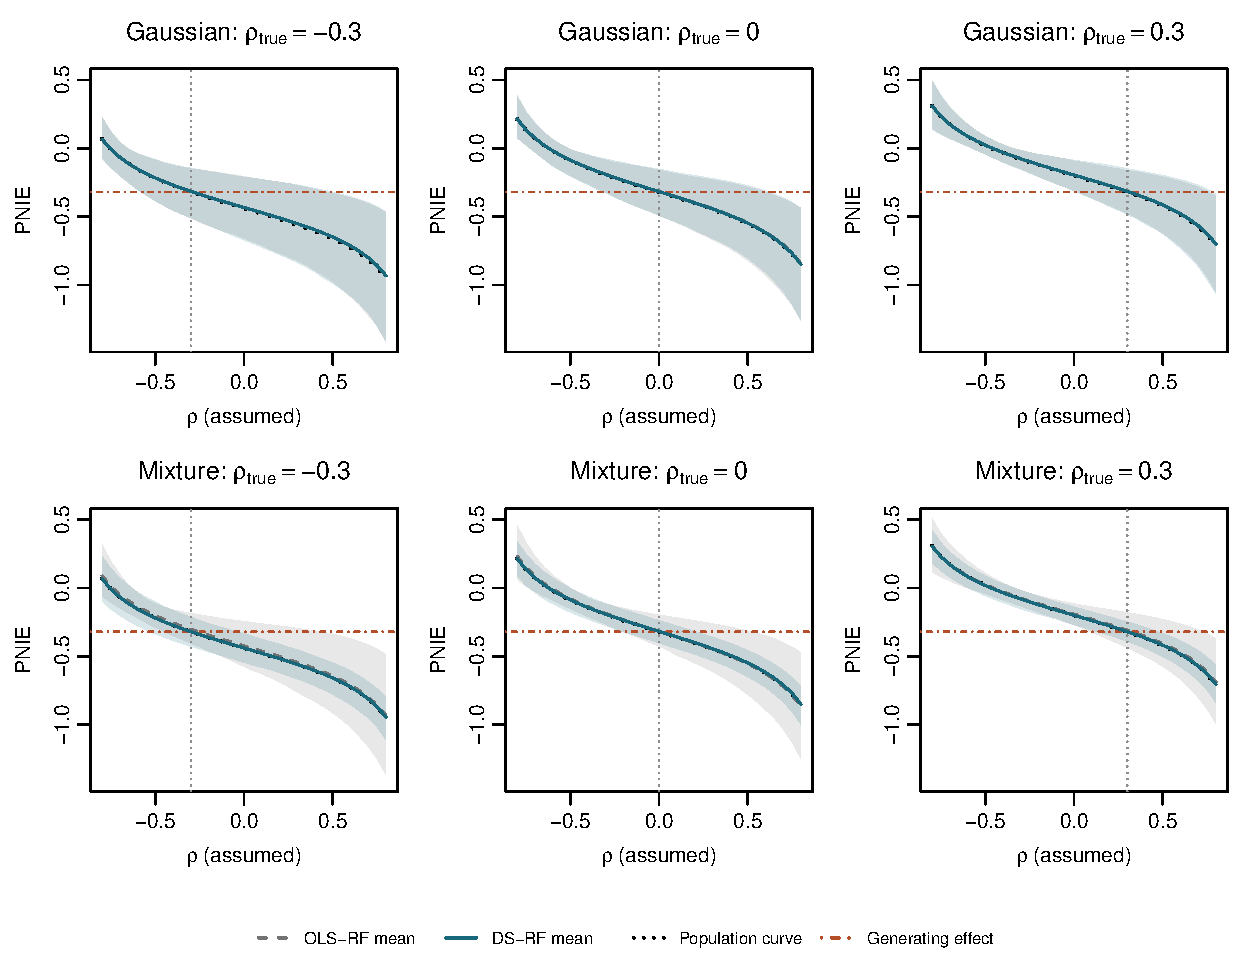
\includegraphics[width=0.98\textwidth]{figures/confounding_simulation_curves.pdf}
\caption{Simulated PNIE sensitivity curves at $n=300$, with 500 attempted replications for each generating correlation and innovation density. Lines show Monte Carlo mean estimates and the population sensitivity curve. Gray and blue shading show central 90\% empirical sampling ranges of the OLS-RF and DS-RF estimates across successful replications, respectively. The horizontal reference is the generating PNIE, $-0.32$, and the vertical reference is the generating correlation. All six configurations are shown.}
\label{fig:simulation-sensitivity-curves}
\end{figure}

Across all three generating correlations and the 33-point grid, paired PNIE RMSE ratios range from 0.985 to 1.054 under Gaussian innovations and from 0.341 to 1.363 under asymmetric-mixture innovations. The asymmetric-mixture results identify regions with substantial precision gains alongside regions with comparable or higher RMSE. Mixture TNIE ratios similarly range from 0.367 to 1.085. This pattern is explained by the nuisance components that dominate the effect gradient: near a zero of $b_t(\rho)$, the derivative of $\delta_t$ with respect to $\beta_2$ is small, whereas regions with a larger derivative can benefit more from precise mediator treatment-effect estimation.

For mixture innovations, DS-RF pointwise curve coverage ranges from 0.924 to 0.966 for PNIE and from 0.904 to 0.964 for TNIE, quantifying the calibration accompanying the precision pattern across the grid. Gaussian coverage likewise varies with the assumed correlation. Zero-boundary RMSE and interval lengths are nearly identical between methods (Table~S11), as predicted by their shared first-order residual-moment representation. Together, the results characterize three complementary features of sensitivity analysis: precision along the assumed-correlation curve, pointwise interval calibration and the point-estimate zero boundary. The separately retained generating-effect inclusion frequencies quantify how recovery of the causal effect depends on the specified confounding value.

\FloatBarrier

